\makebox[\columnwidth][c]{
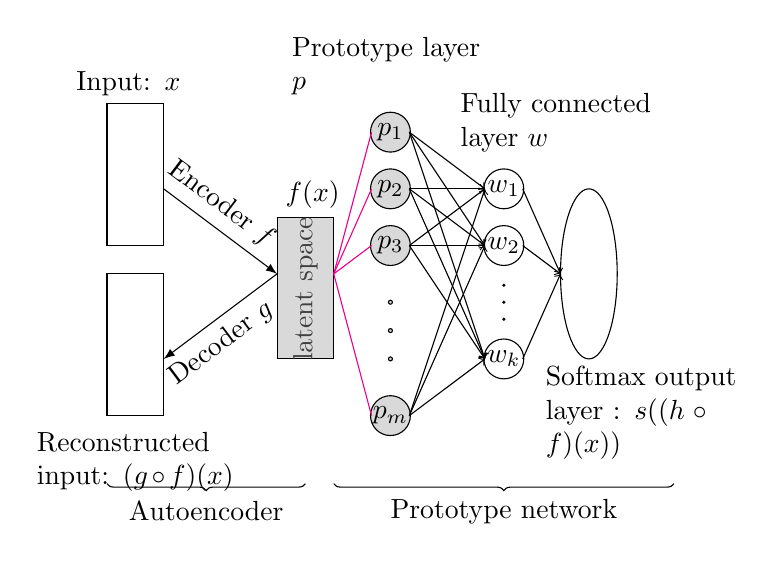
\begin{tikzpicture}[scale=0.72]
  \filldraw[fill=white, draw=black] (0,0) rectangle (1,2.5) ;
  \path (0,0) -- (1,2.5) node[midway, below,  yshift=-2.8em, text width=2.5cm] {Reconstructed input: $(g \circ f)(\bm{x})$ };
  \filldraw[fill=white, draw=black] (0,3) rectangle (1,5.5);
  \path (0,3) -- (1,5.5) node[midway, above, yshift=2.5em, text width=1.5cm] {Input: $\bm{x}$ };
;
\filldraw[fill=gray!30, draw=black] (3,1) rectangle (4,3.5);
\path (3,2) -- (4,4) node[midway, above, yshift=1em, xshift=0.75cm, text width=2cm]{ $f(\bm{x})$} node[color=darkgray,rotate=90,midway,xshift=-0.55cm] {latent space};
\path[-latex] (3, 2.5) edge node [xshift=-0.2cm, sloped, below] {Decoder $g$} (1,1) ;
\path[-latex] (1, 4) edge node [xshift=-0.2cm, sloped, above] {Encoder $f$} (3,2.5);
\coordinate (p1) at (5,0);
\coordinate (p2) at (5,2);
\coordinate (p3) at (5,3);
\coordinate (p4) at (5,4);
\coordinate (pn) at (5,5);
\coordinate (o1) at (7,1);
\coordinate (o2) at (7,2);
\coordinate (o3) at (7,3);
\coordinate (o4) at (7,4);
\filldraw[fill=gray!30, draw=black] (p1) circle (1em) node {$p_m$};
\filldraw[fill=gray!30, draw=black] (p2) circle (0.1em);
\filldraw[fill=gray!30, draw=black] (5,1.5) circle (0.1em);
\filldraw[fill=gray!30, draw=black] (5,1) circle (0.1em);
\filldraw[fill=gray!30, draw=black] (p3) circle (1em) node {$p_3$};
\filldraw[fill=gray!30, draw=black] (p4) circle (1em) node {$p_2$};
\filldraw[fill=gray!30, draw=black] (pn) circle (1em) node {$p_1$}  node[above, yshift=1em, text width=2.5cm] {Prototype layer $p$};
\filldraw[fill=white, draw=black] (o1) circle (1em) node {$w_k$};
\filldraw[fill=gray!30, draw=black] (7,2) circle (0.05em);
\filldraw[fill=gray!30, draw=black] (7,2-0.3) circle (0.05em);
\filldraw[fill=gray!30, draw=black] (7,2+0.3) circle (0.05em);
\filldraw[fill=white, draw=black] (o3) circle (1em) node {$w_2$};
\filldraw[fill=white, draw=black] (o4) circle (1em)node {$w_1$} node [above,yshift=1em, text width=2.5cm, xshift=2em] {Fully connected layer $w$};
 \foreach \i [evaluate=\i as \itext using int(\i)] in {0,3,4,5}
 {
    \path[color=magenta] (4.6666, \i) edge (4,2.5);
    \foreach \j [evaluate=\j as \itext using int(\j)]in {1,3,4}
    {
      \path[->] (5.333, \i) edge (6.666666666666, \j);
    }
  }
\filldraw[fill=white, draw=black] (8.5,2.5) ellipse (0.5 and 1.5) node[below,yshift=-3em, text width=2.5cm, xshift=2em] {Softmax output layer : $s((h\circ f)(\bm{x}))$};
  \foreach \j [evaluate=\j as \itext using int(\j)]in {1,3,4}
    {
      \path[->] (7.333, \j) edge (8, 2.5);
    }

    \draw [decorate,decoration={brace,mirror}] (0,-1.2) -- (3.5,-1.2) node[midway,yshift=-10pt]{Autoencoder};

    \draw [decorate,decoration={brace,mirror}] (4,-1.2) -- (10,-1.2) node[midway,yshift=-10pt]{Prototype network};
\end{tikzpicture}}
